\documentclass{article}

\usepackage{amsmath}
\usepackage{xcolor}
\usepackage{graphicx}
\usepackage[margin=1in]{geometry}
\usepackage{tikz}
\usepackage{listings}
\usepackage{hyperref}

\lstset{
    basicstyle=\ttfamily,
    language=Prolog
}
\title{CS 571 Project 6 Instructions}
\date{ }

\newcommand{\todo}[1]{\textbf{\textcolor{red}{#1}}}

\begin{document}
\maketitle
\section*{Due Monday, Dec. 8}
\section{Search Problem \hfill 10 points}

In this problem you will consider an agent whose goal is to get to some treasure.
At each time step, the agent can move between rooms using doors arranged according to an undirected graph.
However, some of the doors are locked, and the agent must acquire the appropriate key in order to pass through a locked door.
For example, consider the scenario depicted in the following graph:\\[0.5em]
\begin{minipage}{\textwidth}
\begin{center}
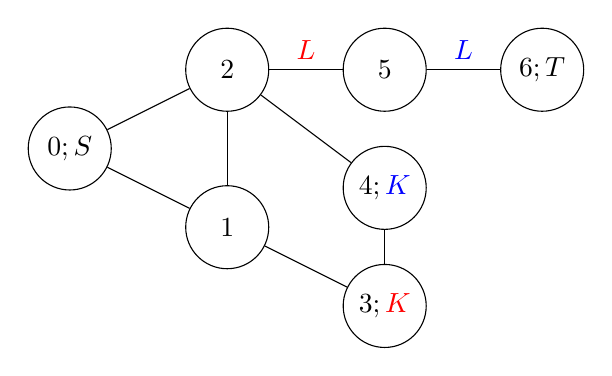
\begin{tikzpicture}
    \draw (0,0) node (node0) [circle,draw,minimum size=3em] {$0; S$};
    \draw (2,-1) node (node1) [circle,draw,minimum size=3em] {$1$};
    \draw (2,1) node (node2) [circle,draw,minimum size=3em] {$2$};
    \draw (4, -2) node (node3) [circle, draw,minimum size=3em] {$3; \textcolor{red}{K}$};
    \draw(4, -0.5) node (node4) [circle, draw,minimum size=3em] {$4; \textcolor{blue}{K}$};
    \draw (4, 1) node (node5) [circle, draw,minimum size=3em] {$5$};
    \draw(6, 1) node (node6) [circle, draw,minimum size=3em] {$6; T$};
    \draw (3, 1.25) node {$\textcolor{red}{L}$};
    \draw (5, 1.25) node {$\textcolor{blue}{L}$};

    \draw (node0) -- (node1);
    \draw (node0) -- (node2);
    \draw (node1) -- (node2);
    \draw (node1) -- (node3);
    \draw (node2) -- (node4);
    \draw (node3) -- (node4);
    \draw (node2) -- (node5);
    \draw (node5) -- (node6);
\end{tikzpicture}
\end{center}
\end{minipage}
In this scenario, the agent starts in room $0$, as indicated by the $S$ annotation.
The treasure is located in room $6$, but the door from room $5$ to $6$ is locked with a blue lock -- as indicated by a blue $\textcolor{blue}{L}$ -- and the door from room $2$ to $5$ is locked with a red lock -- as indicated by a red $\textcolor{red}{L}$.
Thus in order to reach the treasure, the agent must first acquire both the red key -- located in room $3$ as indicated by the red $\textcolor{red}{K}$ -- and the blue key -- located in room $4$ as indicated by the blue $\textcolor{blue}{K}$.
Thus, the shortest path the agent can travel to reach the treasure in this scenario is through the rooms $0,1,3,4,2,5,6$.
This scenario is modeled in Prolog in the file \texttt{search/scenario1.pl}.

\noindent
Your task in this question is to, given a specification of a problem such as the one in \texttt{search/scenario1.pl}, write a search procedure in Prolog to find the shortest path for the agent to reach the treasure.
You should write -- in the file \texttt{search/search.pl} -- a predicate called \lstinline{search(X)} that binds \lstinline{X} to the shortest sequence of moves to lead the agent to the treasure.
Examples of the output format are in \texttt{search/test1.pl} and \texttt{search/test2.pl}.

\section{Parsing in Prolog \hfill 5 points}
Write a parsing algorithm in Prolog for the following grammar, assuming the start nonterminal is $\mathit{Lines}$.
\begin{align*}
    \mathit{Lines} & \rightarrow \mathit{Line} \; \mathit{;} \; \mathit{Lines} \; | \; \mathit{Line}\\
    \mathit{Line} & \rightarrow \mathit{Num} \; \mathit{,} \; \mathit{Line} \; | \; \mathit{Num}\\
    \mathit{Num} & \rightarrow \mathit{Digit} \; | \; \mathit{Digit} \; \mathit{Num}\\
    \mathit{Digit} & \rightarrow 0 \; | \; 1 \; | \; 2 \; | \; 3 \; | \; 4 \; | \; 5 \; | \; 6 \; | \; 7 \; | \; 8 \; | \; 9
\end{align*}
Please write your parser as the predicate \lstinline{parse(X)} that is true if andd only if the input list \lstinline{X} of tokens is in the language specified by the grammar.
Write this in the file \texttt{parsing/parse.pl}, which also contains examples.
For the purpose of this question, you may not use the DCG operator \lstinline{-->}.
\end{document}
